% =================================================

\begin{frame}
\frametitle{Protocol}
\framesubtitle{Protocolls Used in Different Cities}
\begin{figure}
\centering
\missingfigure[figwidth=7cm]{}
\caption{Missing figure caption}
\end{figure}
\end{frame}

% =================================================

\begin{frame}
\frametitle{Data Sources}
\framesubtitle{Overview of Traffic Light Control (Ampelbeeinflussung)}
\begin{figure}
\centering
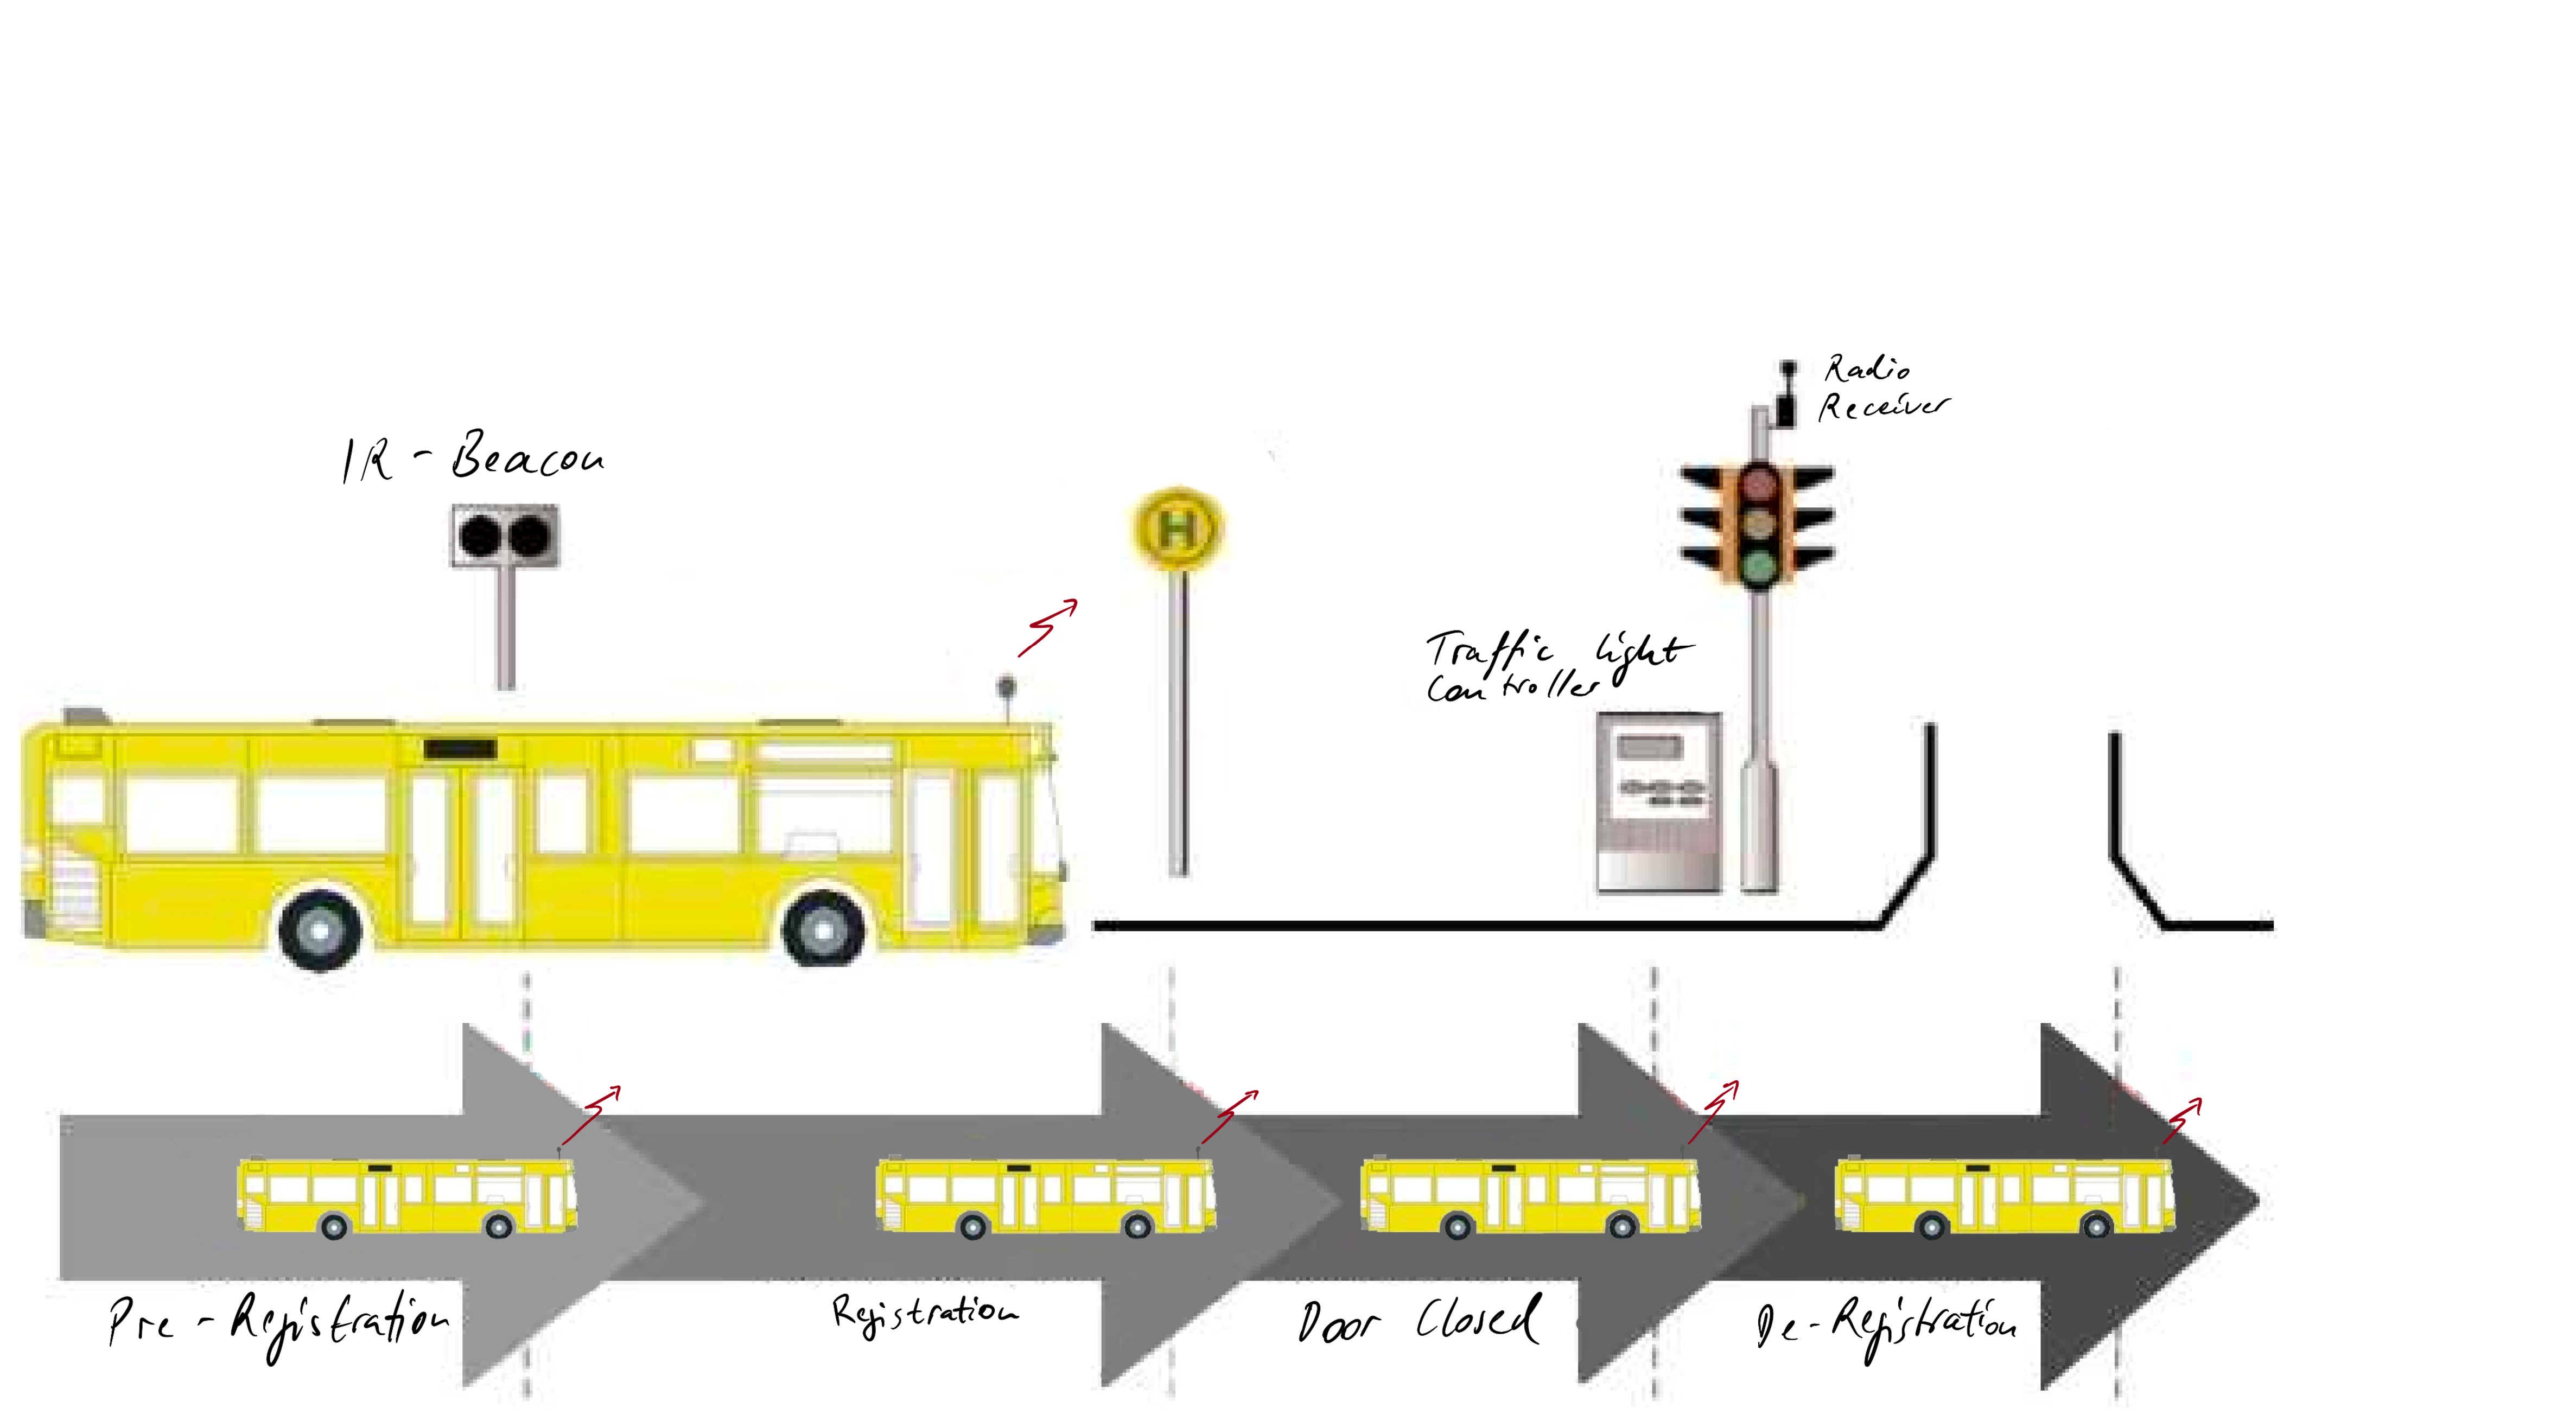
\includegraphics[height=0.65\textheight]{figs/lsa-beeinflussungs-stecke.pdf}
\caption{Traffic light controlled by radio link of busses and trams}
\end{figure}
\end{frame}

% =================================================

\begin{frame}
\frametitle{Data Sources}
\framesubtitle{Overview of Traffic Light Control (Ampelbeeinflussung)}
\begin{figure}
\centering
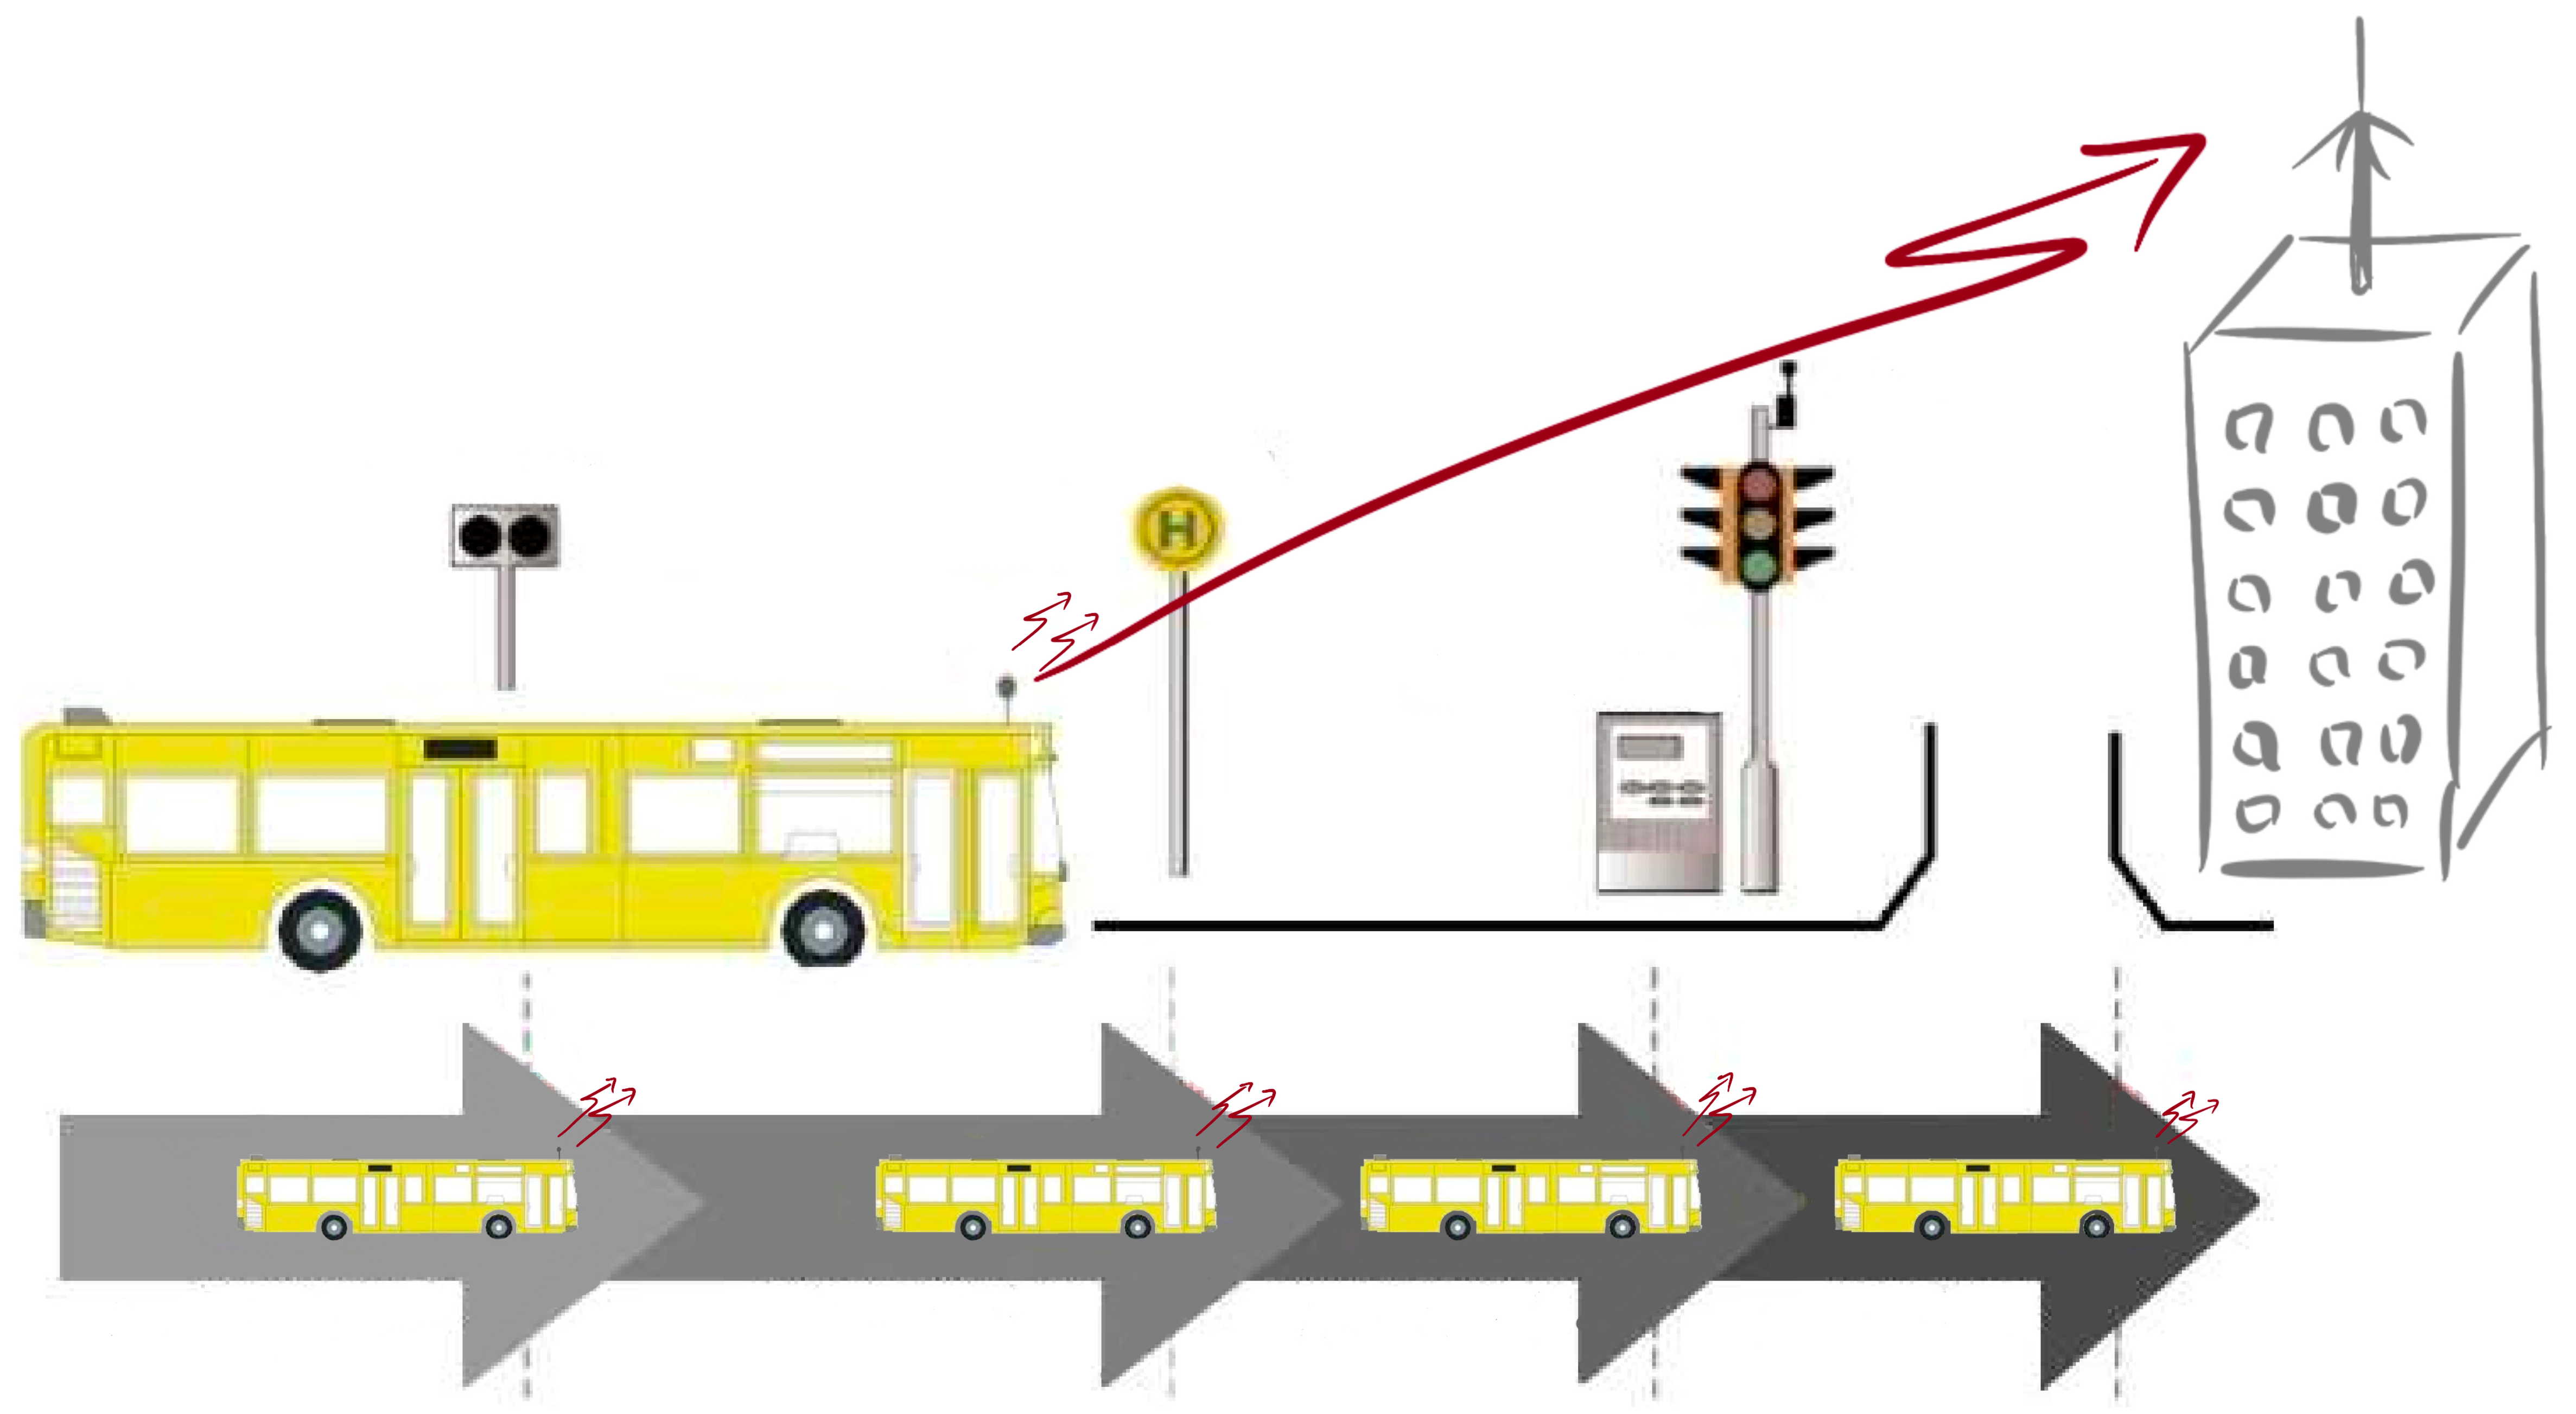
\includegraphics[height=0.65\textheight]{figs/lsa-beeinflussungs-stecke-mit-antenne.pdf}
\caption{Radio signals can be received by our antennas}
\end{figure}
\end{frame}

% =================================================

\begin{frame}
\frametitle{Data Sources}
\framesubtitle{Receiver Overview}
\begin{figure}
\centering
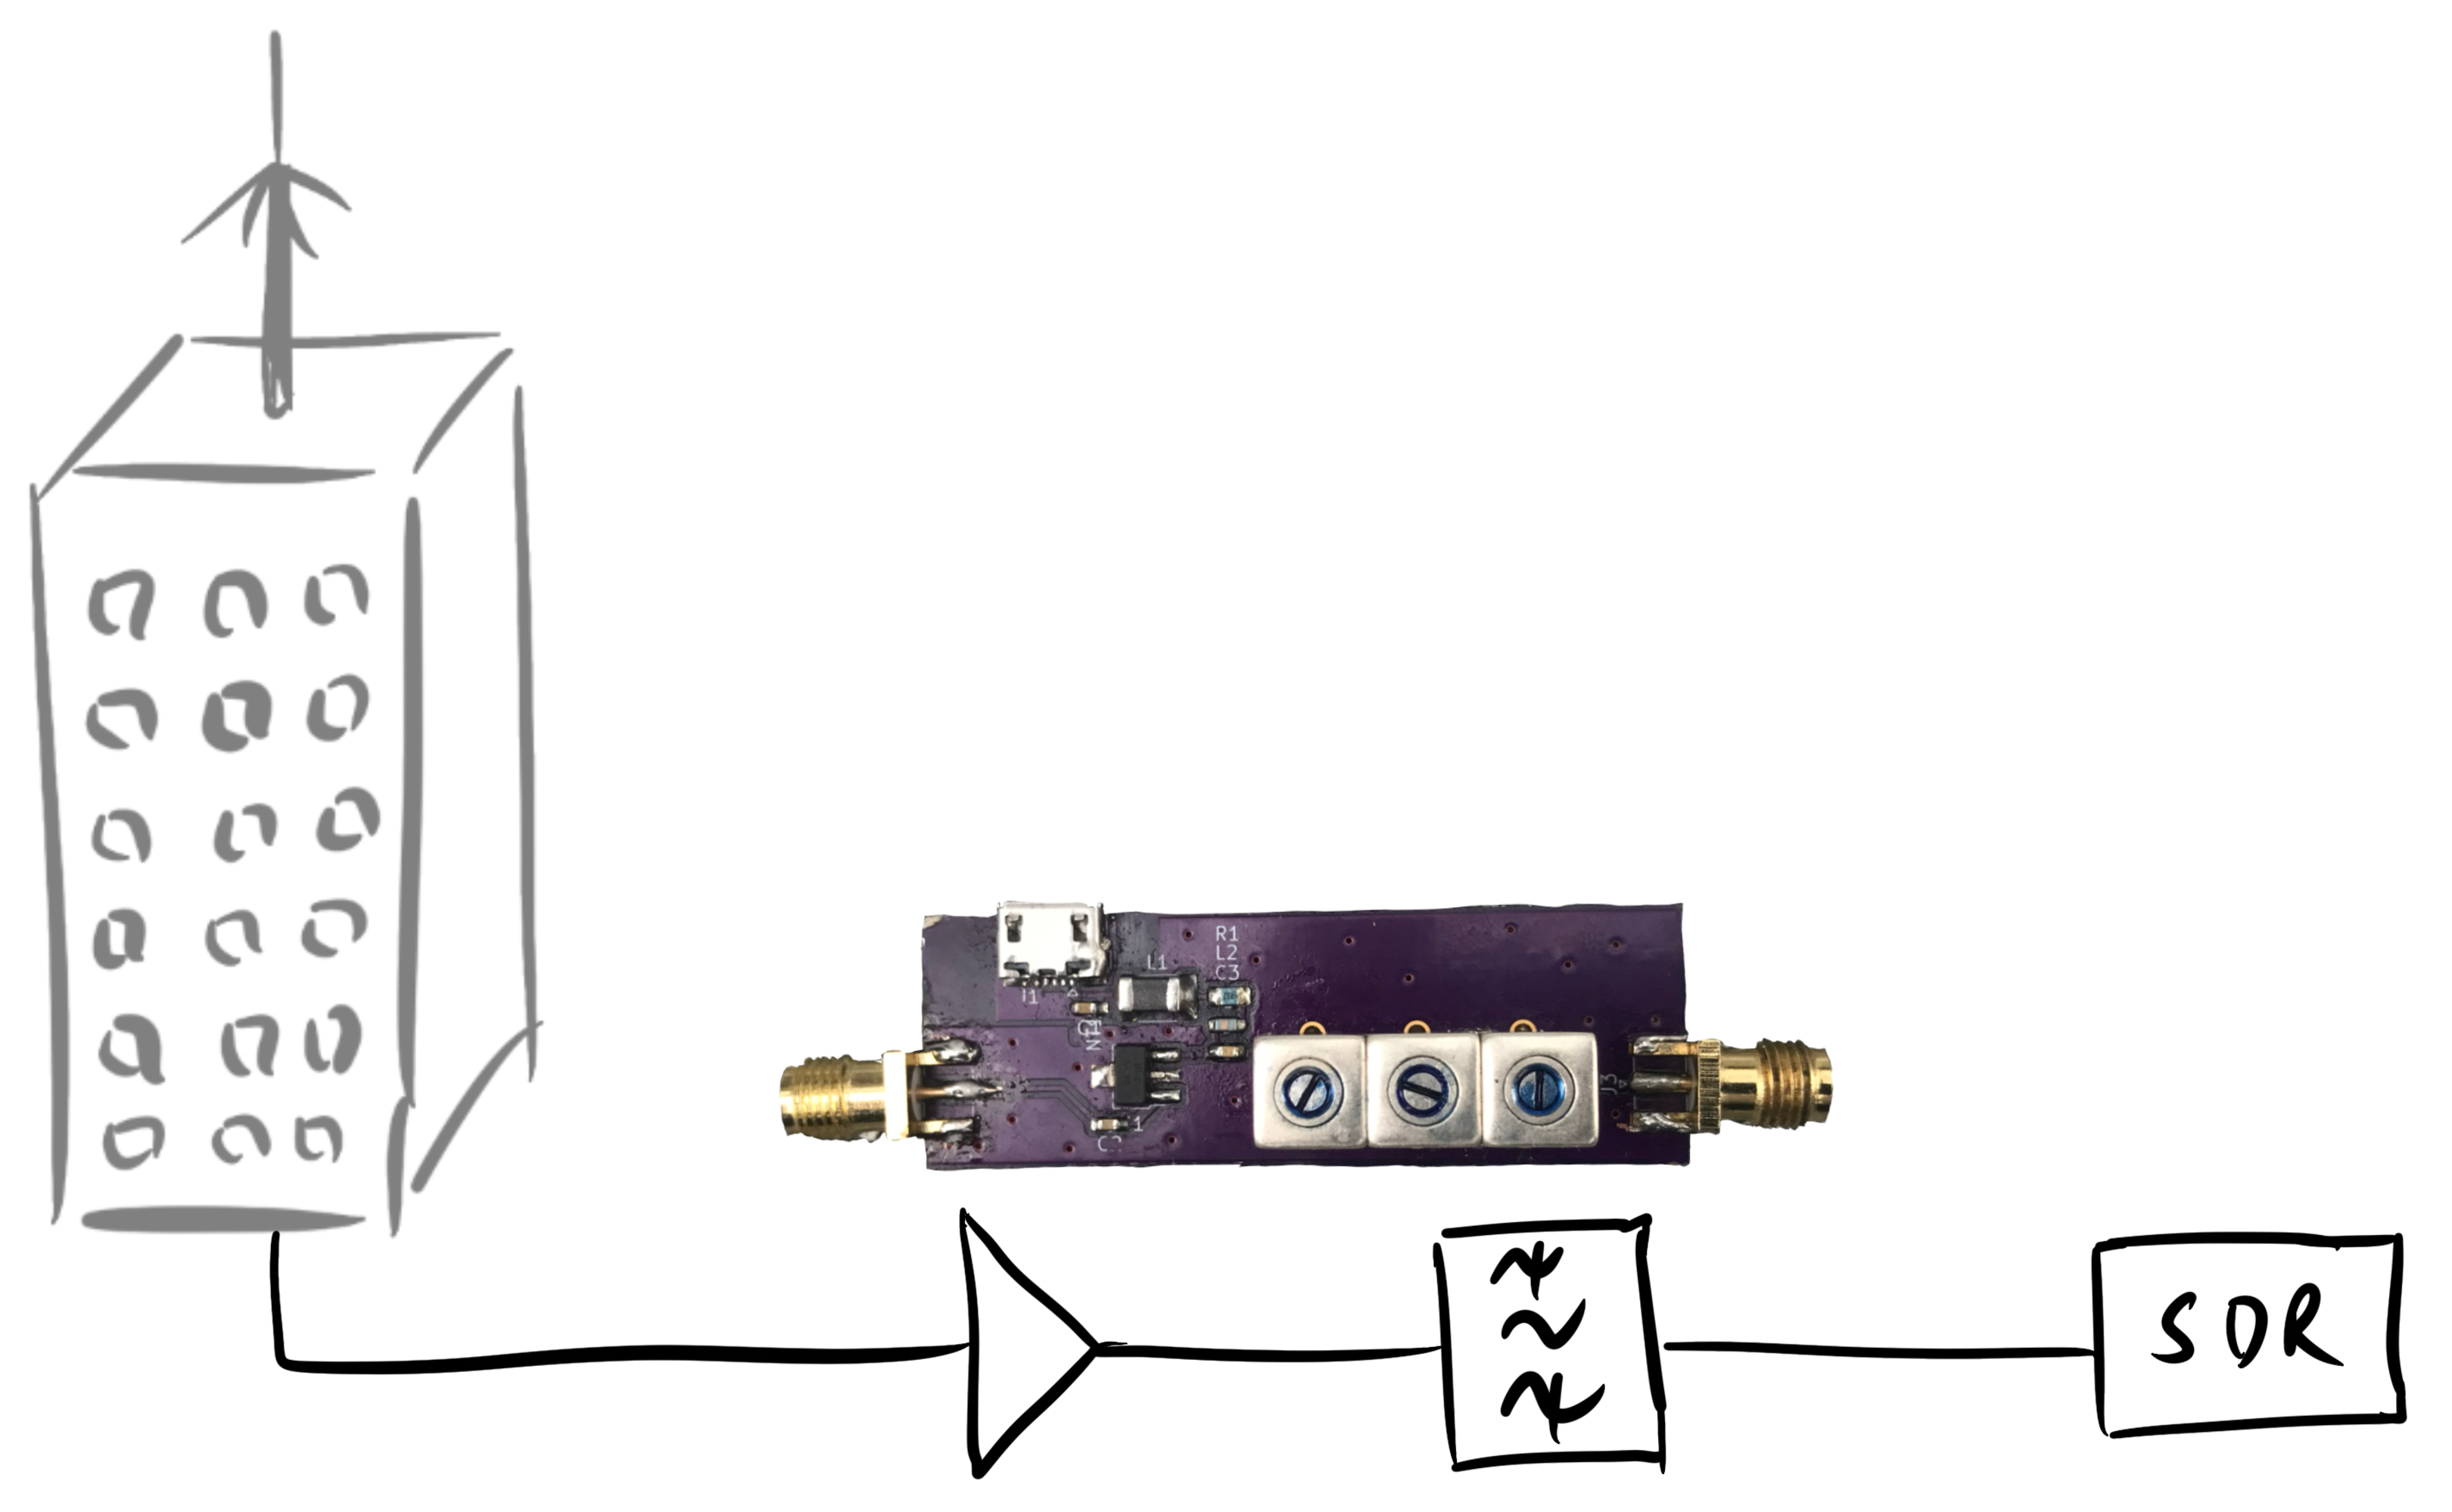
\includegraphics[height=0.65\textheight]{figs/antenna-filter.pdf}
\caption{Schematic overview of the receiver hardware}
\end{figure}
\end{frame}

% =================================================

\begin{frame}
\frametitle{Protocol}
\framesubtitle{VDV 420}
	\begin{itemize}
%		\item which protocol?
%		\item which frequency?
		\item some background on Ampelbeeinflussung and VDV 420 / 426
		\item R09 telegrams of trams and busses standardized in \href{https://knowhow.vdv.de/documents/420/}{VDV 420}
	\end{itemize}
\end{frame}

% =================================================

\begin{frame}
\frametitle{Protocol}
\framesubtitle{VDV 420 Data}
\begin{itemize}
	\item what data can we receive?
	\begin{itemize}
		\item Tram identification data: line number (3 BCD), run number (2 BCD), destination number (3 BCD)
		\item Location data: traffic light id, direction, registration\_type all in 16 bit
		\item and some other (delay)
	\end{itemize}
\end{itemize}
\end{frame}

% =================================================

\begin{frame}
\frametitle{Protocol}
\framesubtitle{VDV 420 Physical Layer}
\begin{columns}
\column{0.6\linewidth}
\centering
\begin{figure}
\centering
\begin{subfigure}[b]{0.46\textwidth}
	\centering
	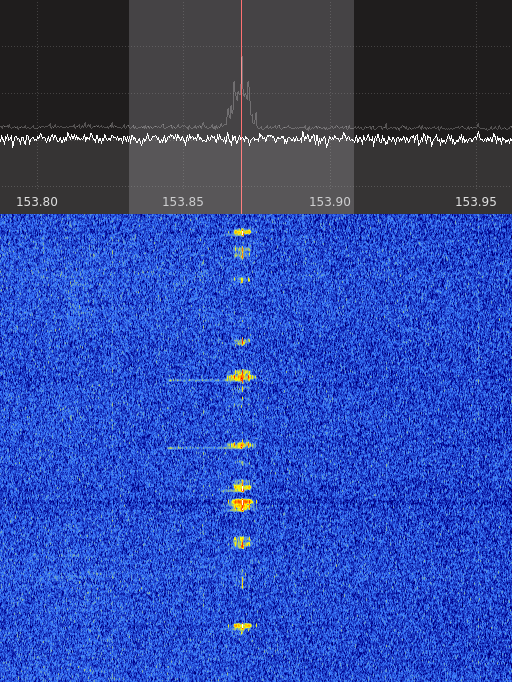
\includegraphics[height=0.65\textheight,width=\textwidth]{figs/spectrum_chemnitz_cropped.png}
\end{subfigure}
\hfill
\begin{subfigure}[b]{0.46\textwidth}
	\centering
	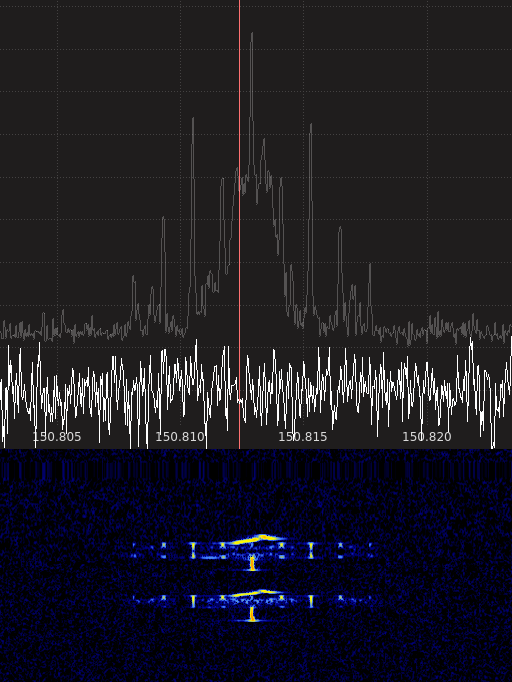
\includegraphics[height=0.65\textheight,width=\textwidth]{figs/spectrum_dresden_cropped.png}
\end{subfigure}
\caption{Screenshots of the bursty transmittion pattern}
\end{figure}
\column{0.4\linewidth}
\begin{itemize}
	\item Bursty transmittion
	\item Minimum Shift Keying with \SI{2400}{Baud}
\end{itemize}
\end{columns}
\end{frame}

% =================================================

\begin{frame}
\frametitle{Protocol}
\framesubtitle{Frequency Identification}
\begin{itemize}
		\item What are the frequency ranges to look for the signal?
		\item Technical documentation of different receivers, i.e. \href{https://www.piciorgros.com/fileadmin/documents/RBL380.pdf}{RBL-380} or \href{https://www.img-nordhausen.de/wp-content/uploads/2021/05/DA\_WZLSA\_2-3\_G\_d\_03\_15.pdf}{WZ LSA 2-3/G}, provide these details
		\item Frequency 70cm Band \SI{450}{\MHz} -- \SI{470}{\MHz}		
		\item Frequency 2m Band \SI{146}{\MHz} -- \SI{174}{\MHz}
		\item Frequency 4m Band \SI{68}{\MHz} -- \SI{87.5}{\MHz}
		\item We have a \href{https://docs.dvb.solutions/chapter\_3\_data\_providers.html}{table of known frequencies}
		\item OSINT: Search for R09 frequency <city>
\end{itemize}
\end{frame}

% =================================================

\begin{frame}
\frametitle{Protocol}
\framesubtitle{Physical Layer Used in Different Cities}
\begin{figure}
% https://opus4.hbz-nrw.de/opus45-bast/frontdoor/deliver/index/docId/2595/file/V353+BF+Gesamtversion.pdf
% page 25
\begin{columns}
\column{.5\linewidth}
\centering
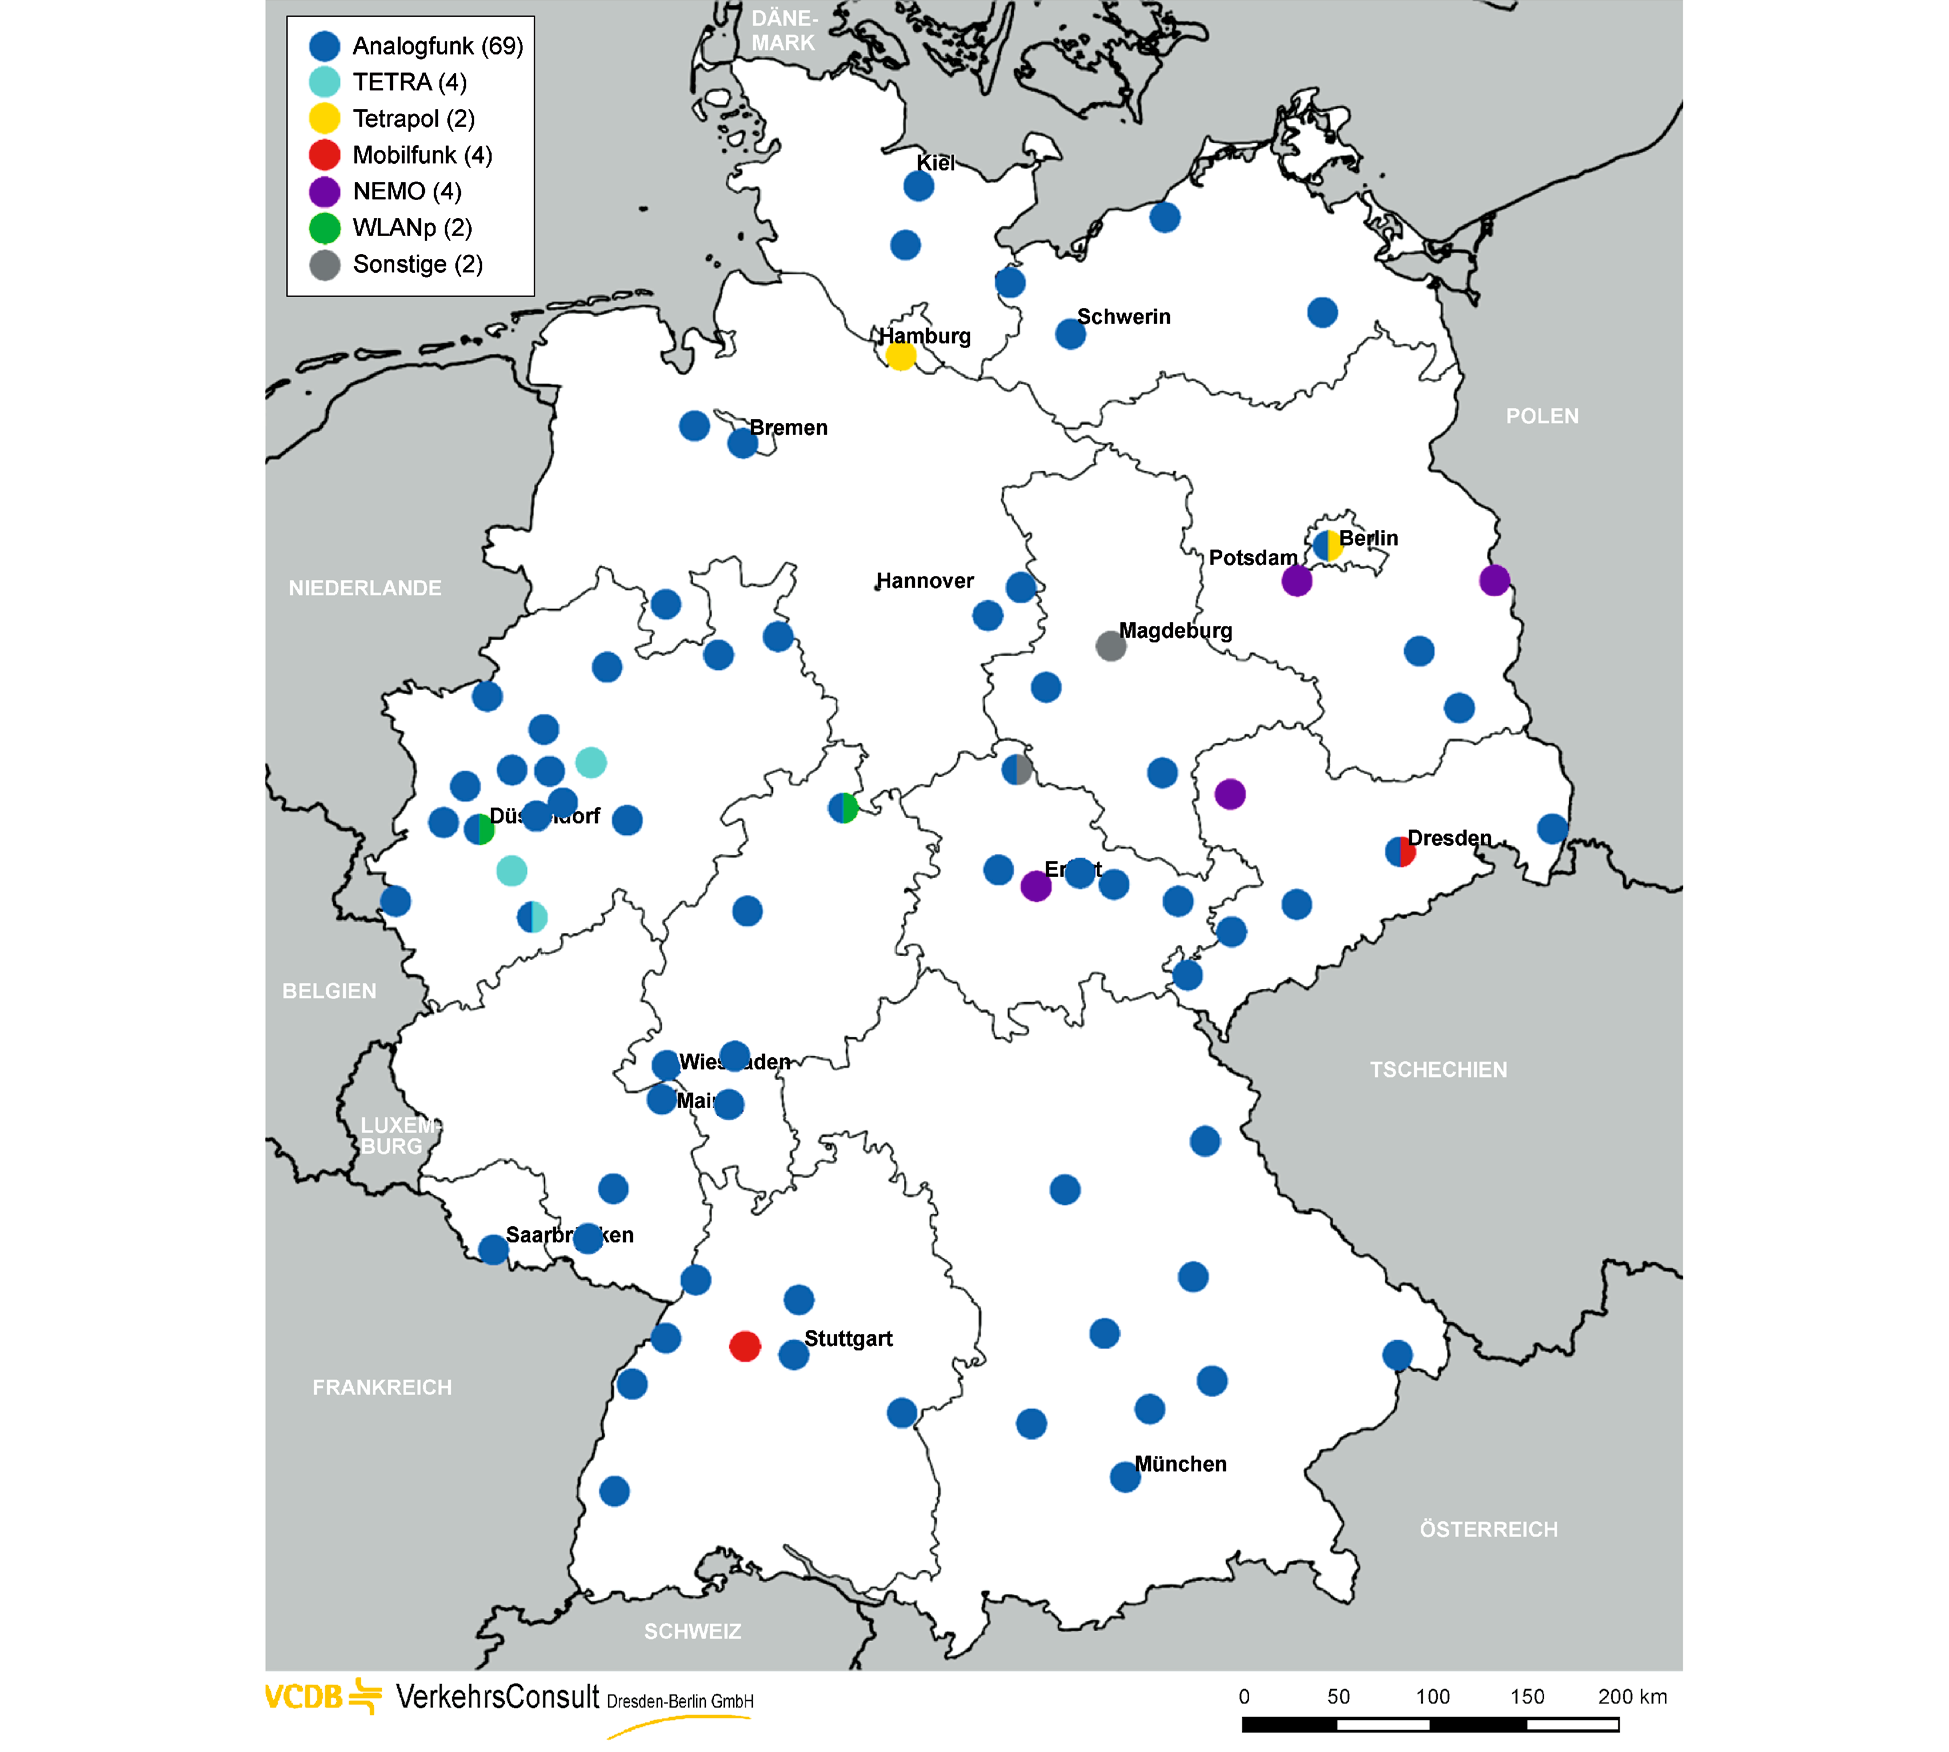
\includegraphics[height=0.8\textheight]{figs/vcdb-map-ampelbeeinflussung.png}
\column{.5\linewidth}
\caption{Map with selected locations which have traffic lights, controlled by public transport. Blue points use the standard we implemented.}
\vspace{0.5cm}
\begin{itemize}
	\item different physical layer protocols described in VDV 426
\end{itemize}
\end{columns}
\end{figure}
\end{frame}

% =================================================
